\section{Block Level Description} \label{sec:block_level}
This section contains block level descriptions of all parts of the system seen in Fig. \ref{fig:top_level}. 

\begin{figure}[H]
  \centering
  \captionsetup{justification=centering}
  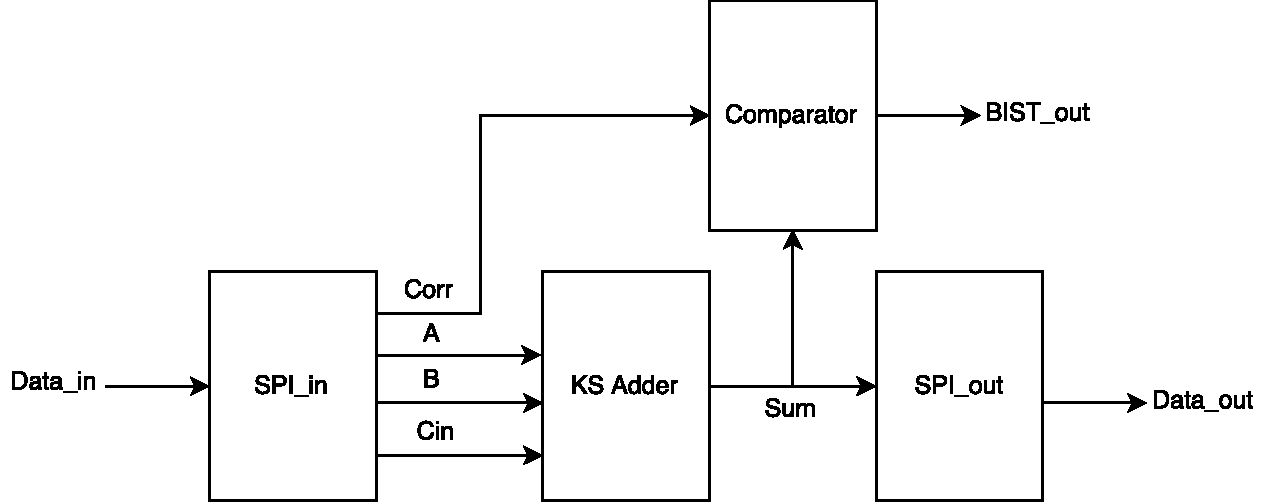
\includegraphics[scale=0.5]{../figures/TOP.pdf}
  \caption{Block diagram of the system.} \label{fig:top_level}
\end{figure}

From the start we were planning on using resettable D flip-flops in the whole system, but after a closer look, we realized that we don't have enough pins to have an external reset. Therefor, we will only be using D flip-flops without reset (with an exeption for a counter in the SPI\_in module, which is reset by the SPI\_enable signal.)


\subsection{SPI-in/PRBS}
The SPI-in (Serial Peripheral Interface - Input) module is supposed to serially receive four times four 16-bit numbers and to distribute the data to the correct parts of the system. The module itself consists of a lot of registers and some control logic moving data between these registers. The PRBS (Pseudo Random Bit Sequence) module is supposed to randomly generate data to the adder in order to be able to test the energy consumption of the system. Since the PRBS module share some registers with the SPI-in module, and the PRBS module is relatively small, we included it as a block in the SPI-in module.

\subsubsection{SPI-receive}
The first block in the SPI-in module is the SPI-receive block (see Fig. \ref{fig:spi_receive}). It consists of 16 D flip-flops (DFF), that is connected one after another in a serial manner. They are clocked on the SPI clock, and on each positive clock edge, a new input bit is shifted in. After 16 pulses we have 16 bits stored, and a load signal is triggered so that each bit is moved to the correct PRBS-register. The order in which the input data arrives can be seen in Fig. \ref{fig:spi_input_data}. As can be seen, the carry in is only one bit, so we use one of the other bits as the check bit for carry out, and one bit to choose if we want to use test or PRBS mode (will be explained later on in this chapter).

\begin{figure}[H]
	\centering
	\captionsetup{justification=centering}
	\includegraphics[scale=0.5]{../figures/SPI_input_data.png}
	\caption{Example of input data} \label{fig:spi_input_data}
\end{figure}

\subsubsection{PRBS-registers}
The PRBS-registers (see Fig. \ref{fig:spi_prbs}) consists of four DFF (one for each addition) and can be run in the following modes:
\begin{itemize}
	\item Read mode
	\item PRBS mode
	\item Test mode
\end{itemize}
 During the first mode the registers are triggered with a load signal, and the data to the first DFF comes from the SPI-receive block. During the second and third mode, the data runs in a feedback loop from the end to the start of the DFF chain and are triggered on the system clock. The SPI\_enable signal determines whether we should read new data or use the feedback loop. The difference between the PRBS and test mode is that during the PRBS mode, the data to the first DFF is the value of the third and forth DFF passed through a XOR, while in test mode, the data to the first DFF is the same as the output from the last DFF. The mode is determined by the value of the test mode signal. Since we only want to check the energy consumption of the adder itself, we have no need to generate random numbers for the checksum. Therefor, the registers that hold the check sum don't need the XOR and the PRBS mode.
 
\subsubsection{SPI\_in controller}
The last block is the control block (see Fig. \ref{fig:spi_controller}), which is the most complex block of the SPI-in module. The heart of the control block is a 6-bit counter. The first four bits signalizes if we have read a 16 bit word or not. The last two bits signalizes which of our four words we are currently reading. By combining these signals like in the figure we are able to produce the load signals that trigger the PRBS-registers.

\begin{figure}[H]
	\centering
	\captionsetup{justification=centering}
	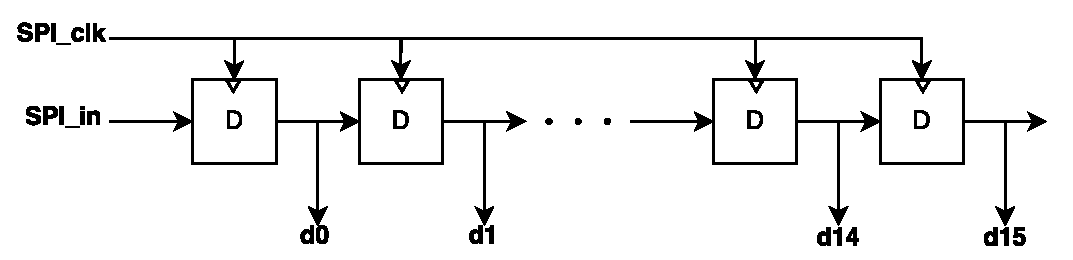
\includegraphics[scale=0.5]{../figures/SPI_receive.pdf}
	\caption{Block diagram of the SPI-receive block.} \label{fig:spi_receive}
\end{figure}

\begin{figure}[H]
	\centering
	\captionsetup{justification=centering}
	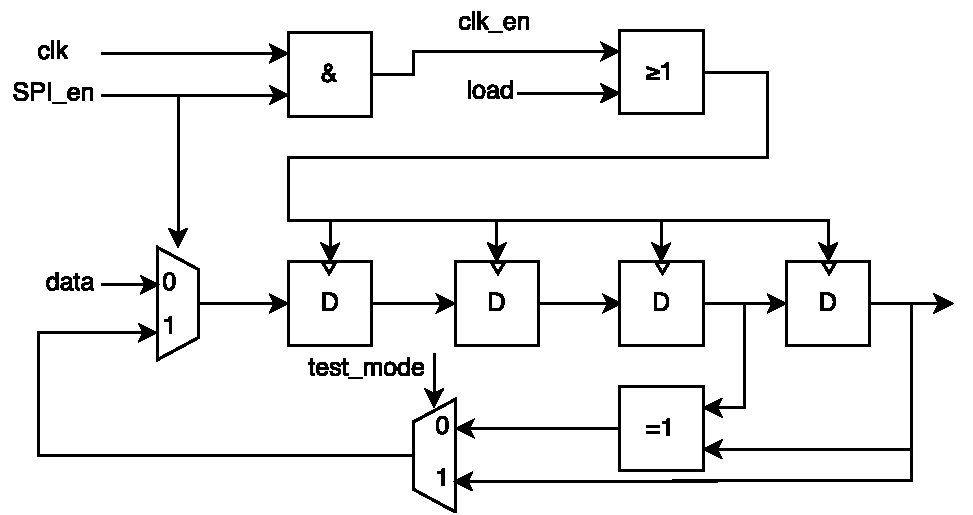
\includegraphics[scale=0.5]{../figures/SPI_PRBS_2.pdf}
	\caption{Block diagram of the SPI-PRBS block.} \label{fig:spi_prbs}
\end{figure}

\begin{figure}[H]
	\centering
	\captionsetup{justification=centering}
	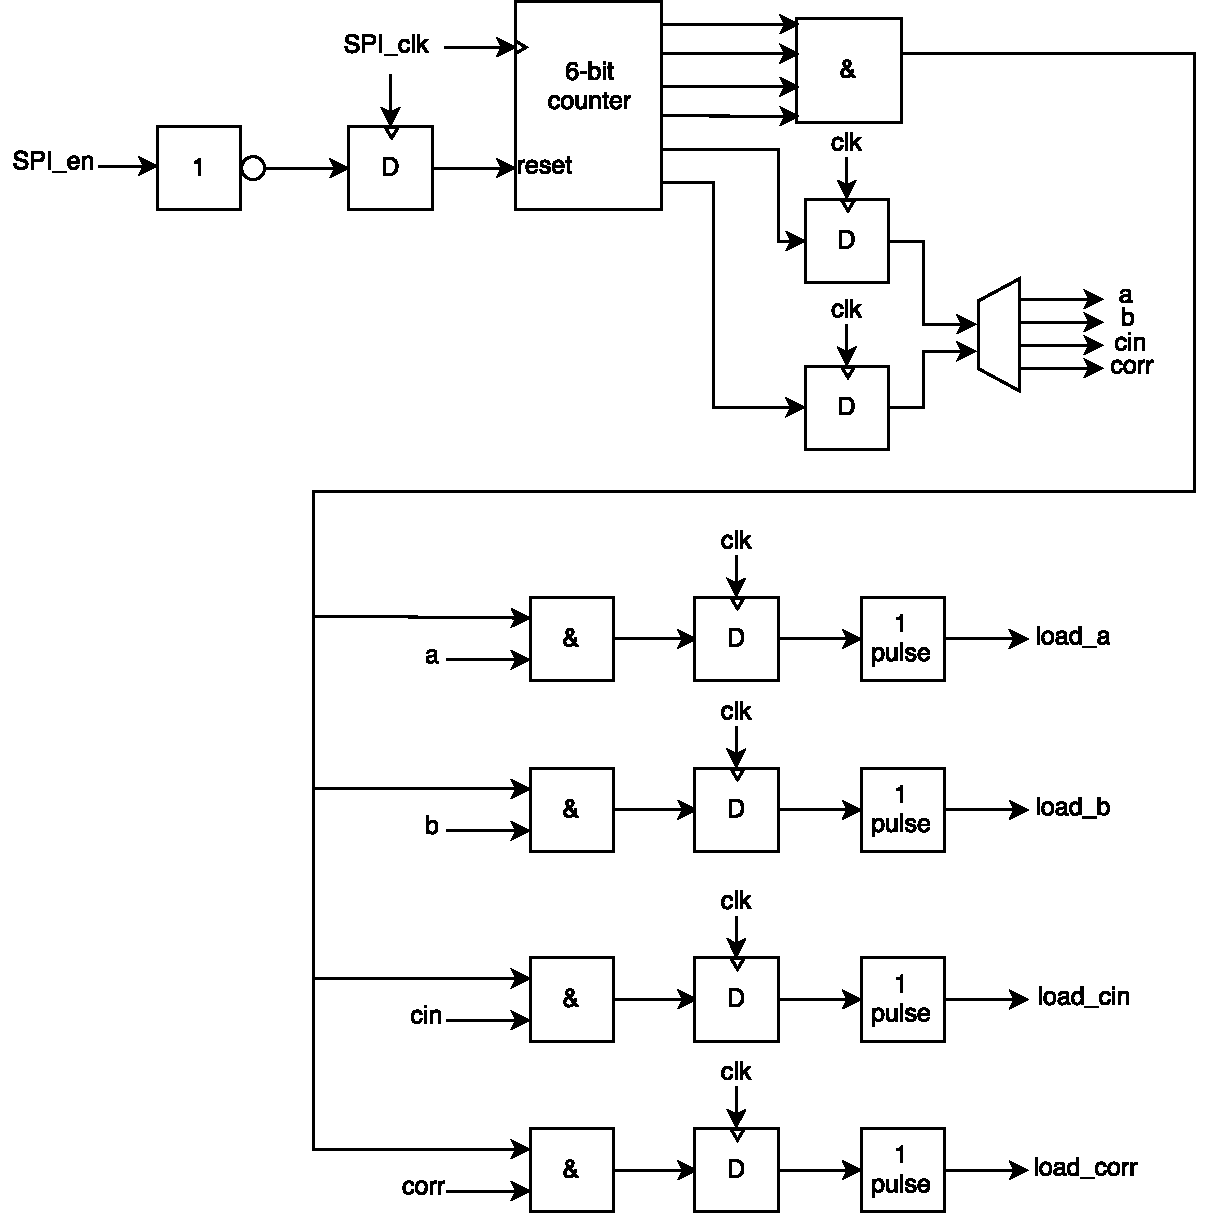
\includegraphics[scale=0.5]{../figures/SPI_controller.pdf}
	\caption{Block diagram of the SPI-controller block.} \label{fig:spi_controller}
\end{figure}

\subsection{16-bit Kogge-Stone Adder}
The Kogge-Stone adder consists of four simple blocks connected in a complex way, as can be seen in appendix \ref{app:ks_block}. These four blocks can be seen in Fig. \ref{fig:red}-\ref{fig:sum}. The red block constitute the initial stage which takes two binary numbers $A$ and $B$ as input. The corresponding truth table is found in table \ref{tab:red} in appendix \ref{app:ks_truth}. The output signals $P$ and $G$ generated from this block are later used by other blocks in the adder. The $G$, also called the Generate signal, trickles down through the hierarchy of the yellow, and the yellow carry blocks to finally end up in the sum block. The truth table for this block can be found in table \ref{tab:sum}. Truth tables for the yellow and yellow carry blocks are found in table \ref{tab:yellow} and \ref{tab:yellowcarry}.

\begin{figure}[H]
  \centering
  \captionsetup{justification=centering}
  \adjustbox{trim={.3\width} {0\height} {.3\width} {0\height},clip}
  {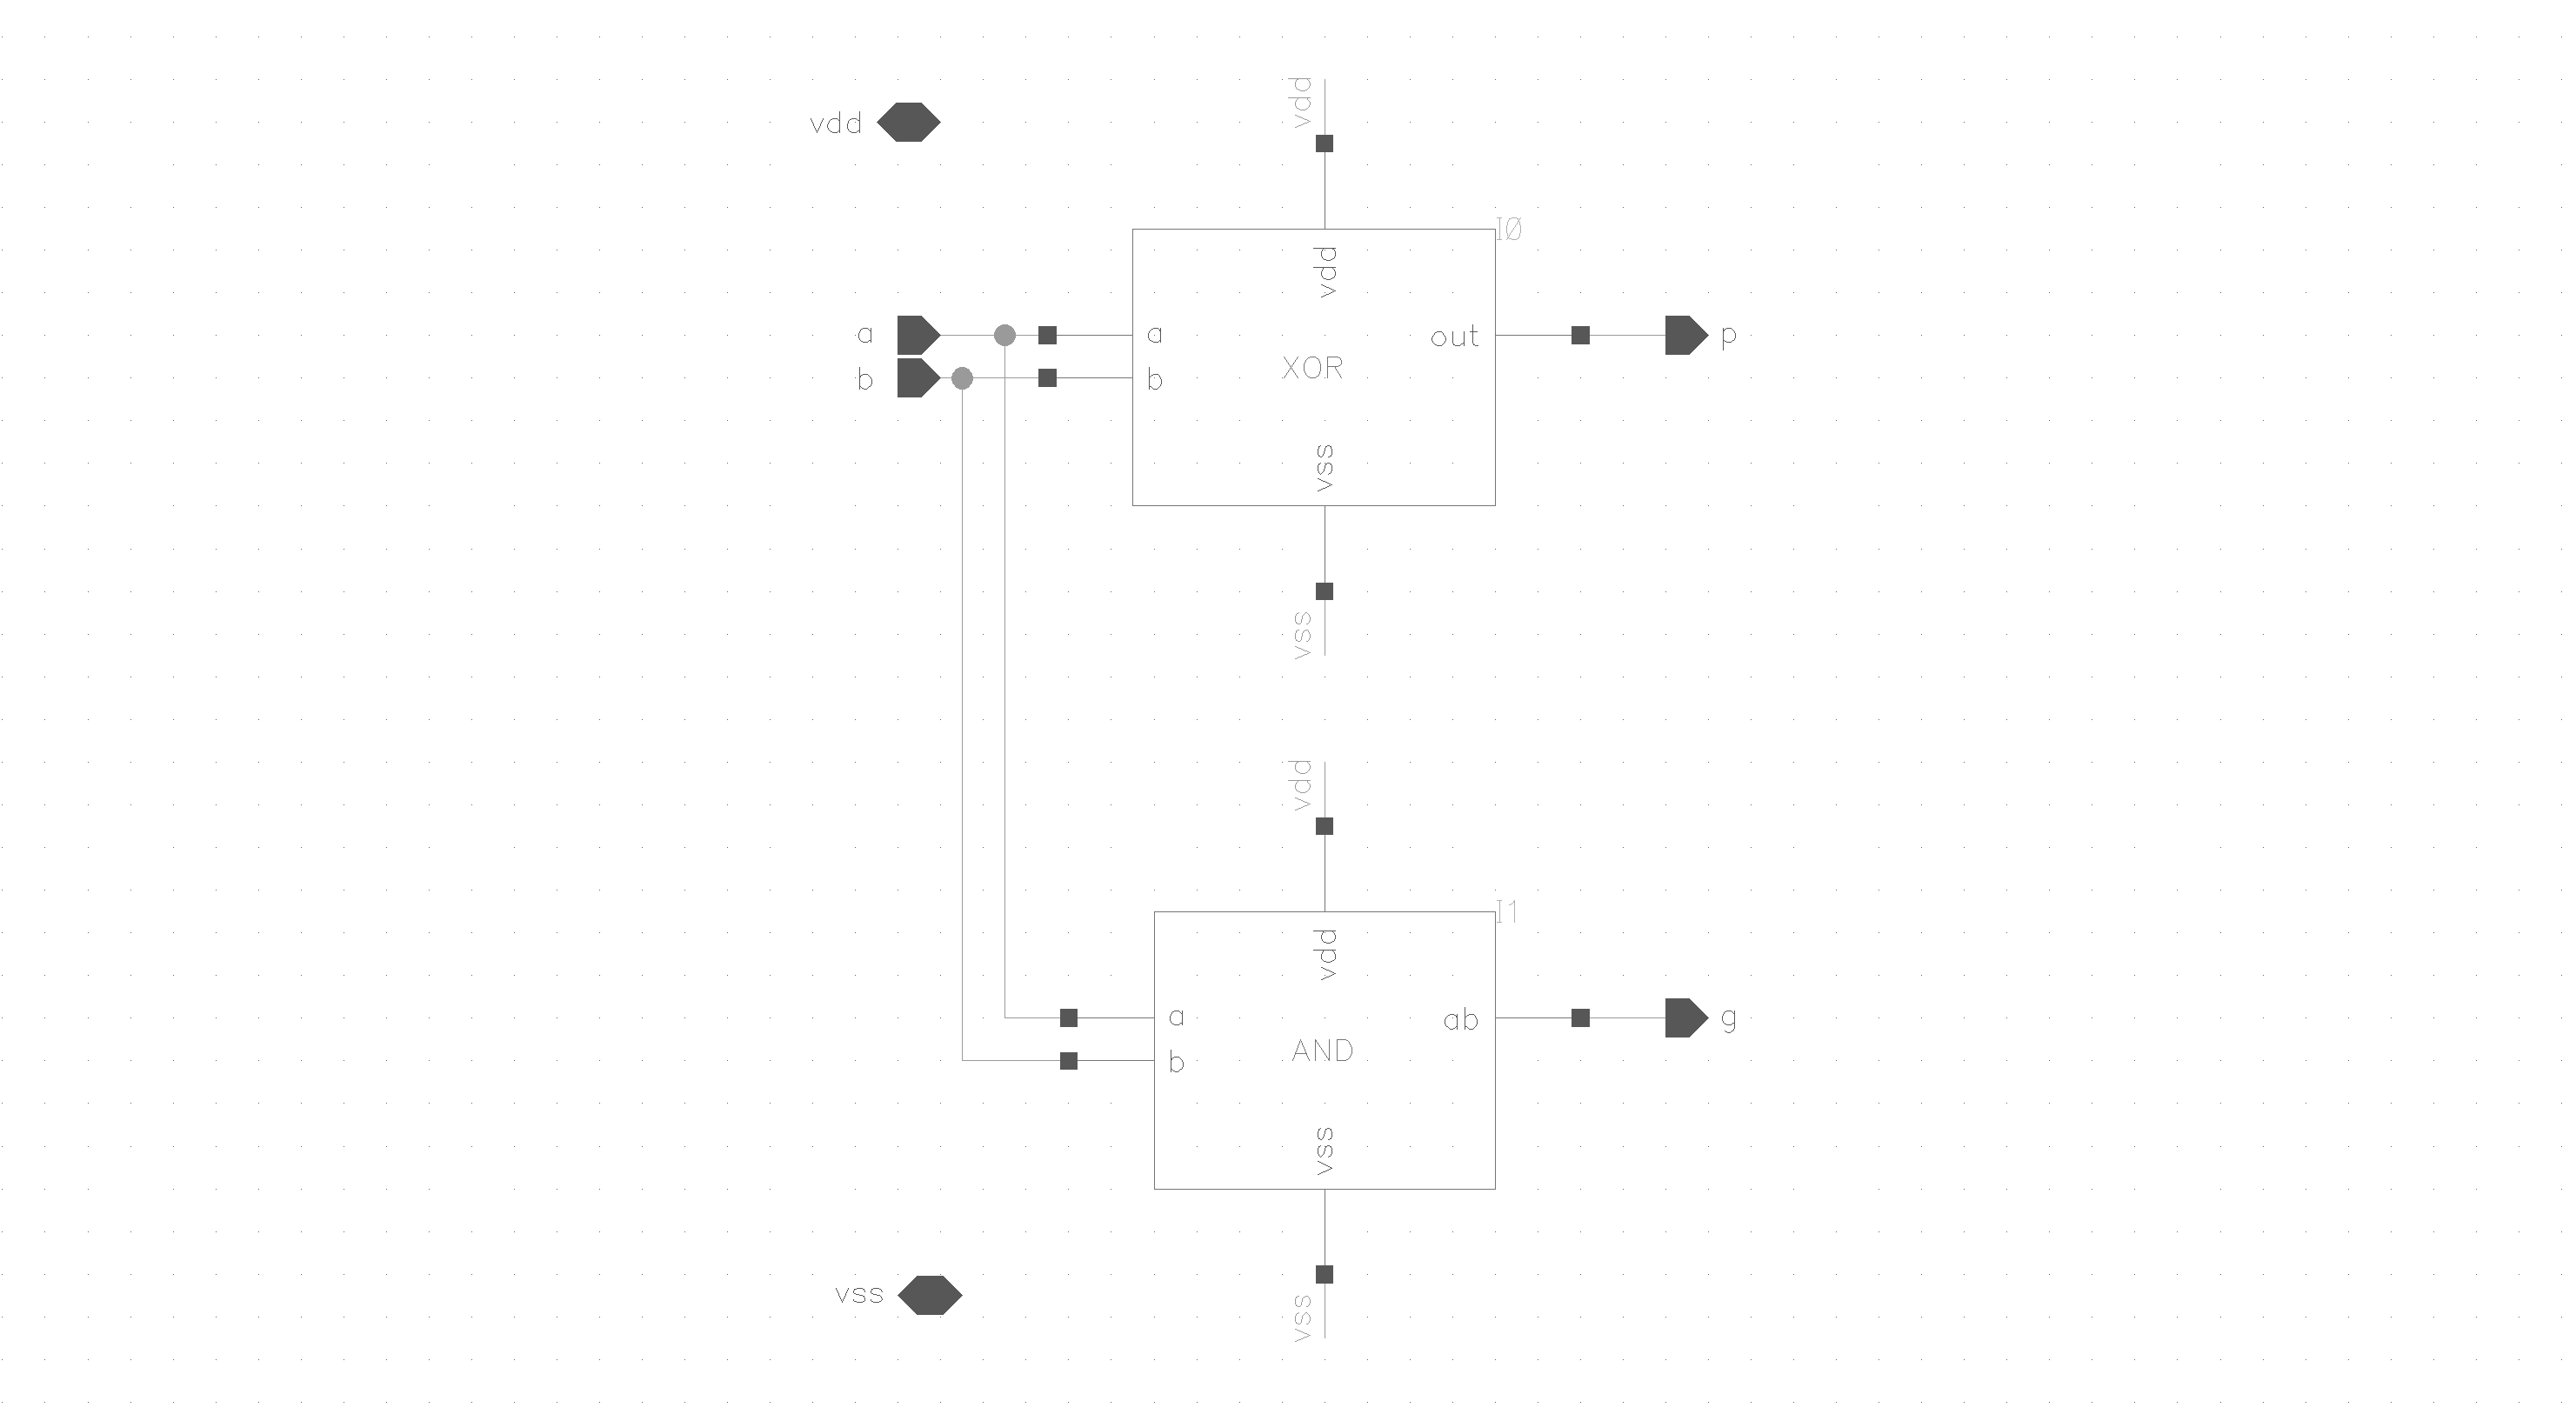
\includegraphics[width=2.0\textwidth]{../figures/red}}
  \caption{Schematic view of the red block.} \label{fig:red}
\end{figure}

\begin{figure}[H]
  \centering
  \captionsetup{justification=centering}
  \adjustbox{trim={.15\width} {0\height} {.12\width} {0\height},clip}
  {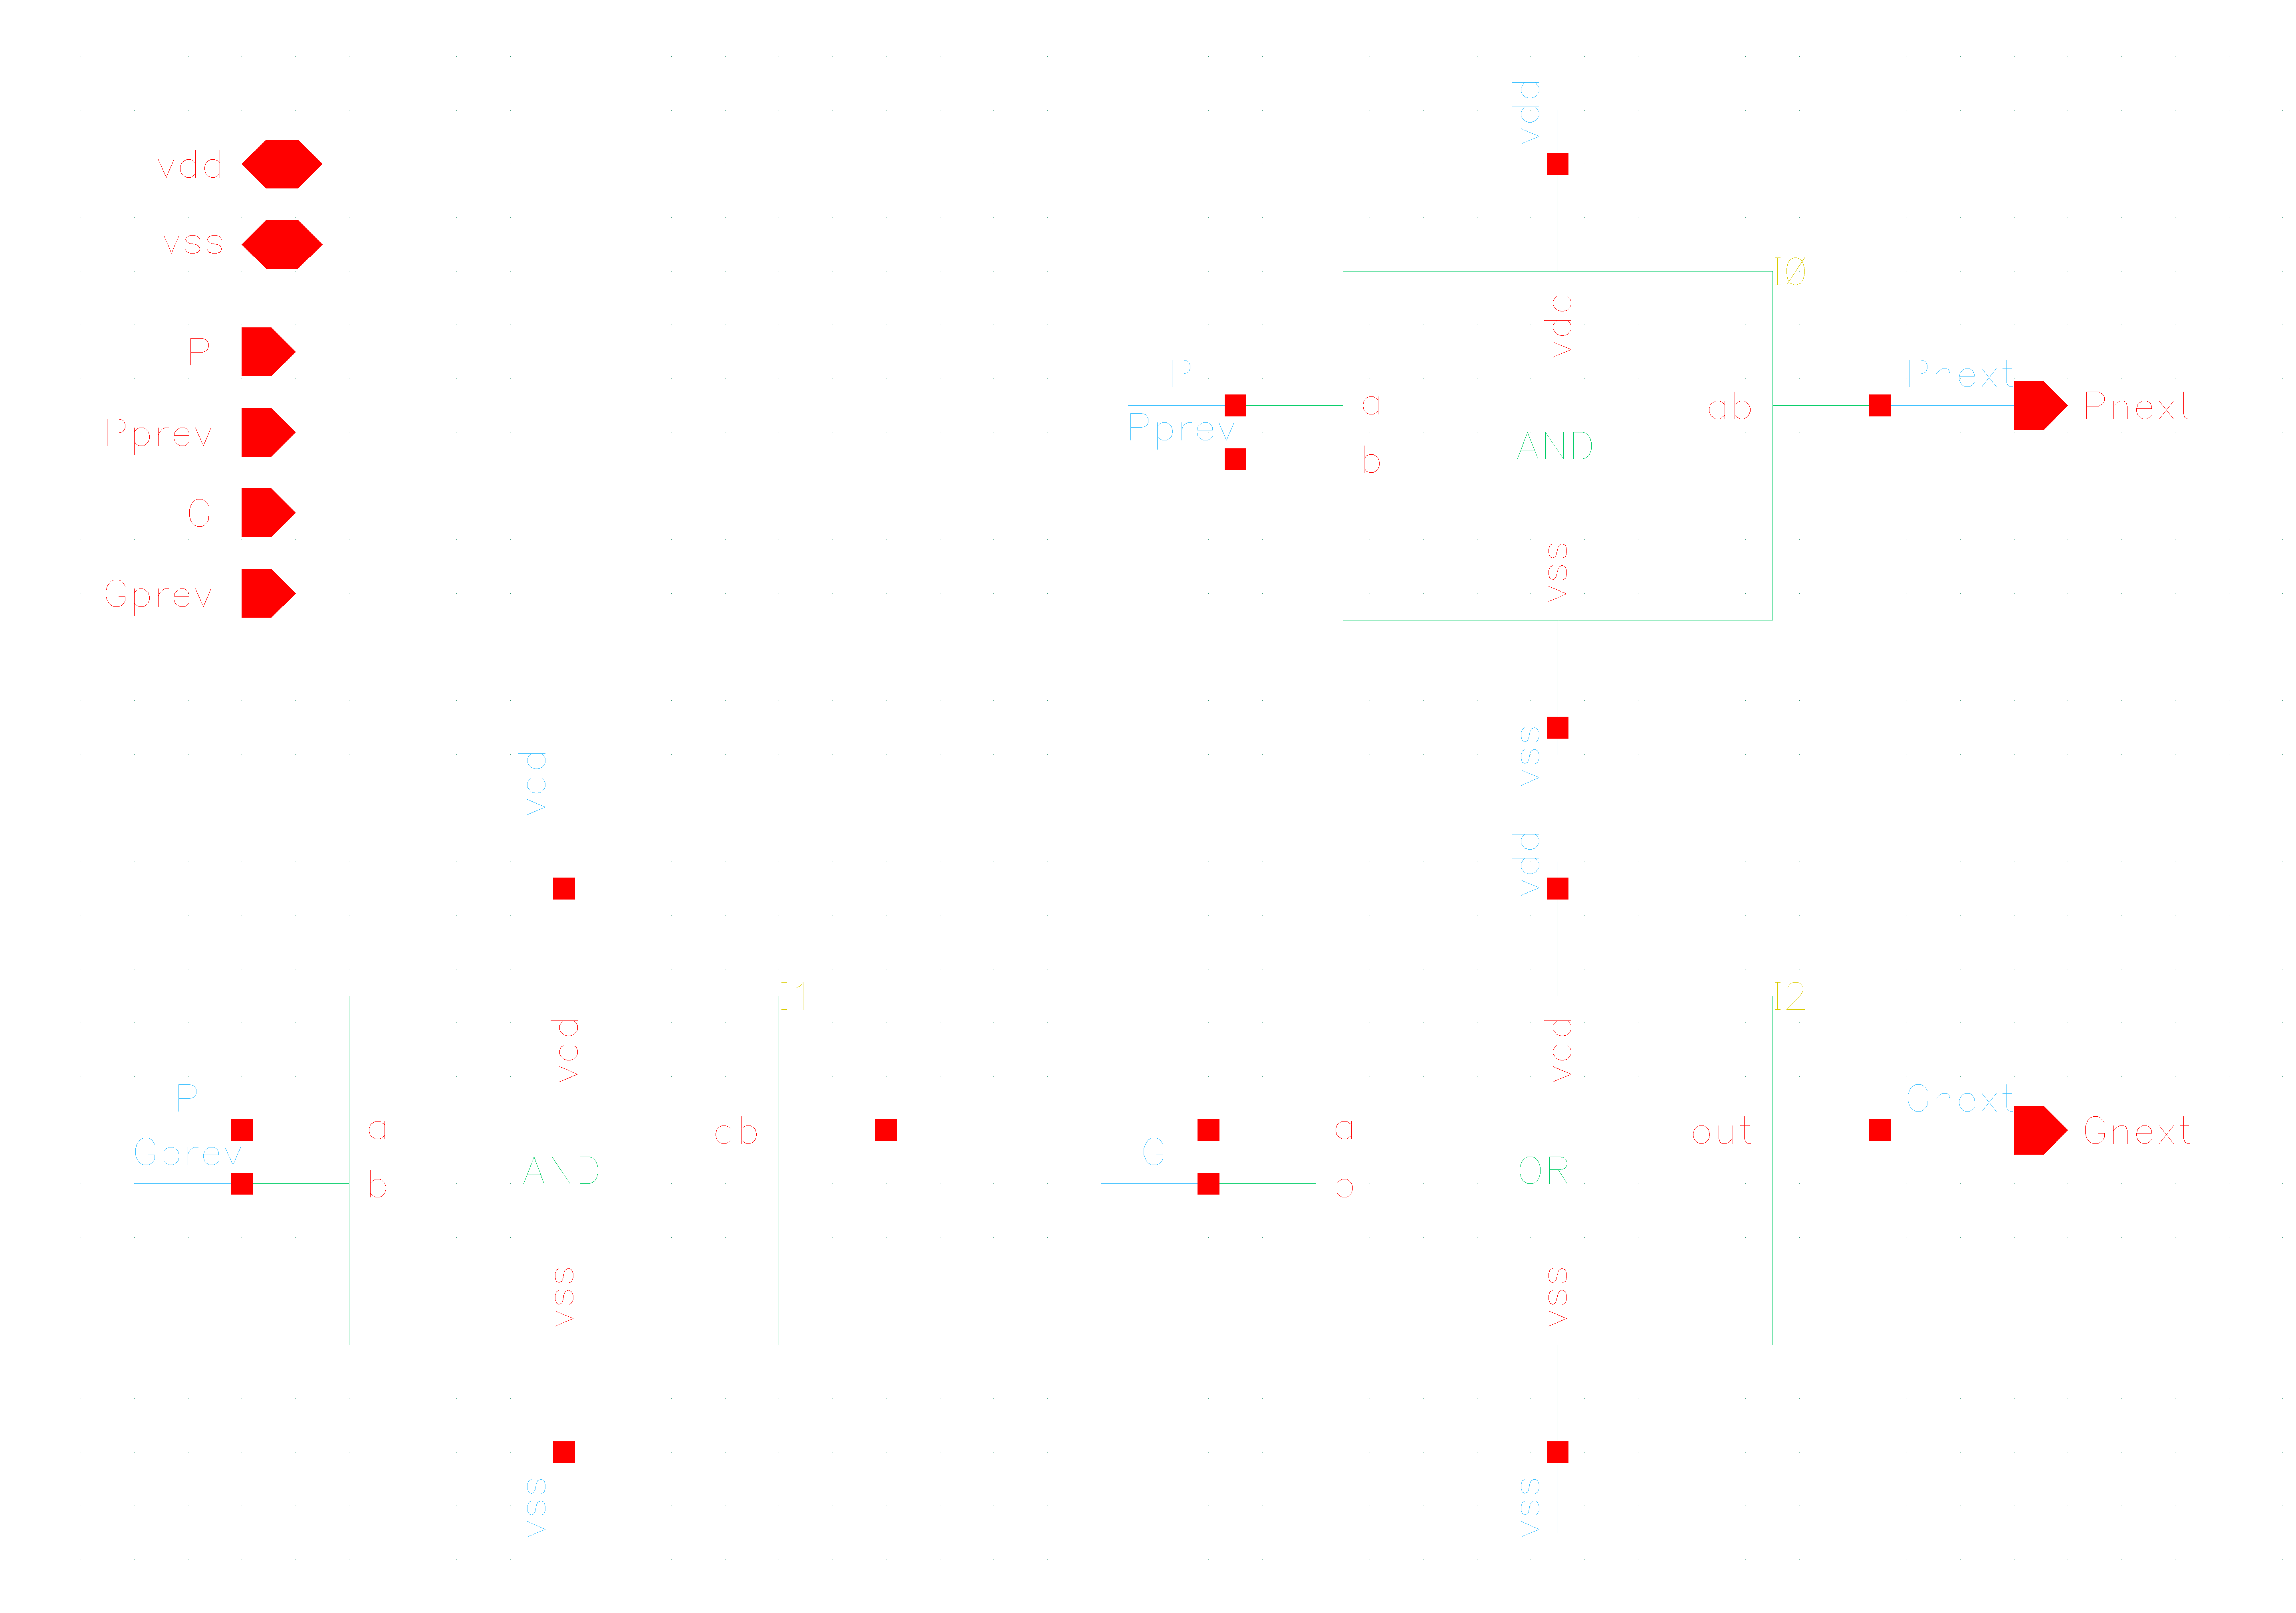
\includegraphics[width=1.3\textwidth]{../figures/yellow}}
  \caption{Schematic view of the yellow block.} \label{fig:yellow}
\end{figure}

\begin{figure}[H]
  \centering
  \captionsetup{justification=centering}
  \adjustbox{trim={.1\width} {0\height} {.1\width} {.4\height},clip}
  {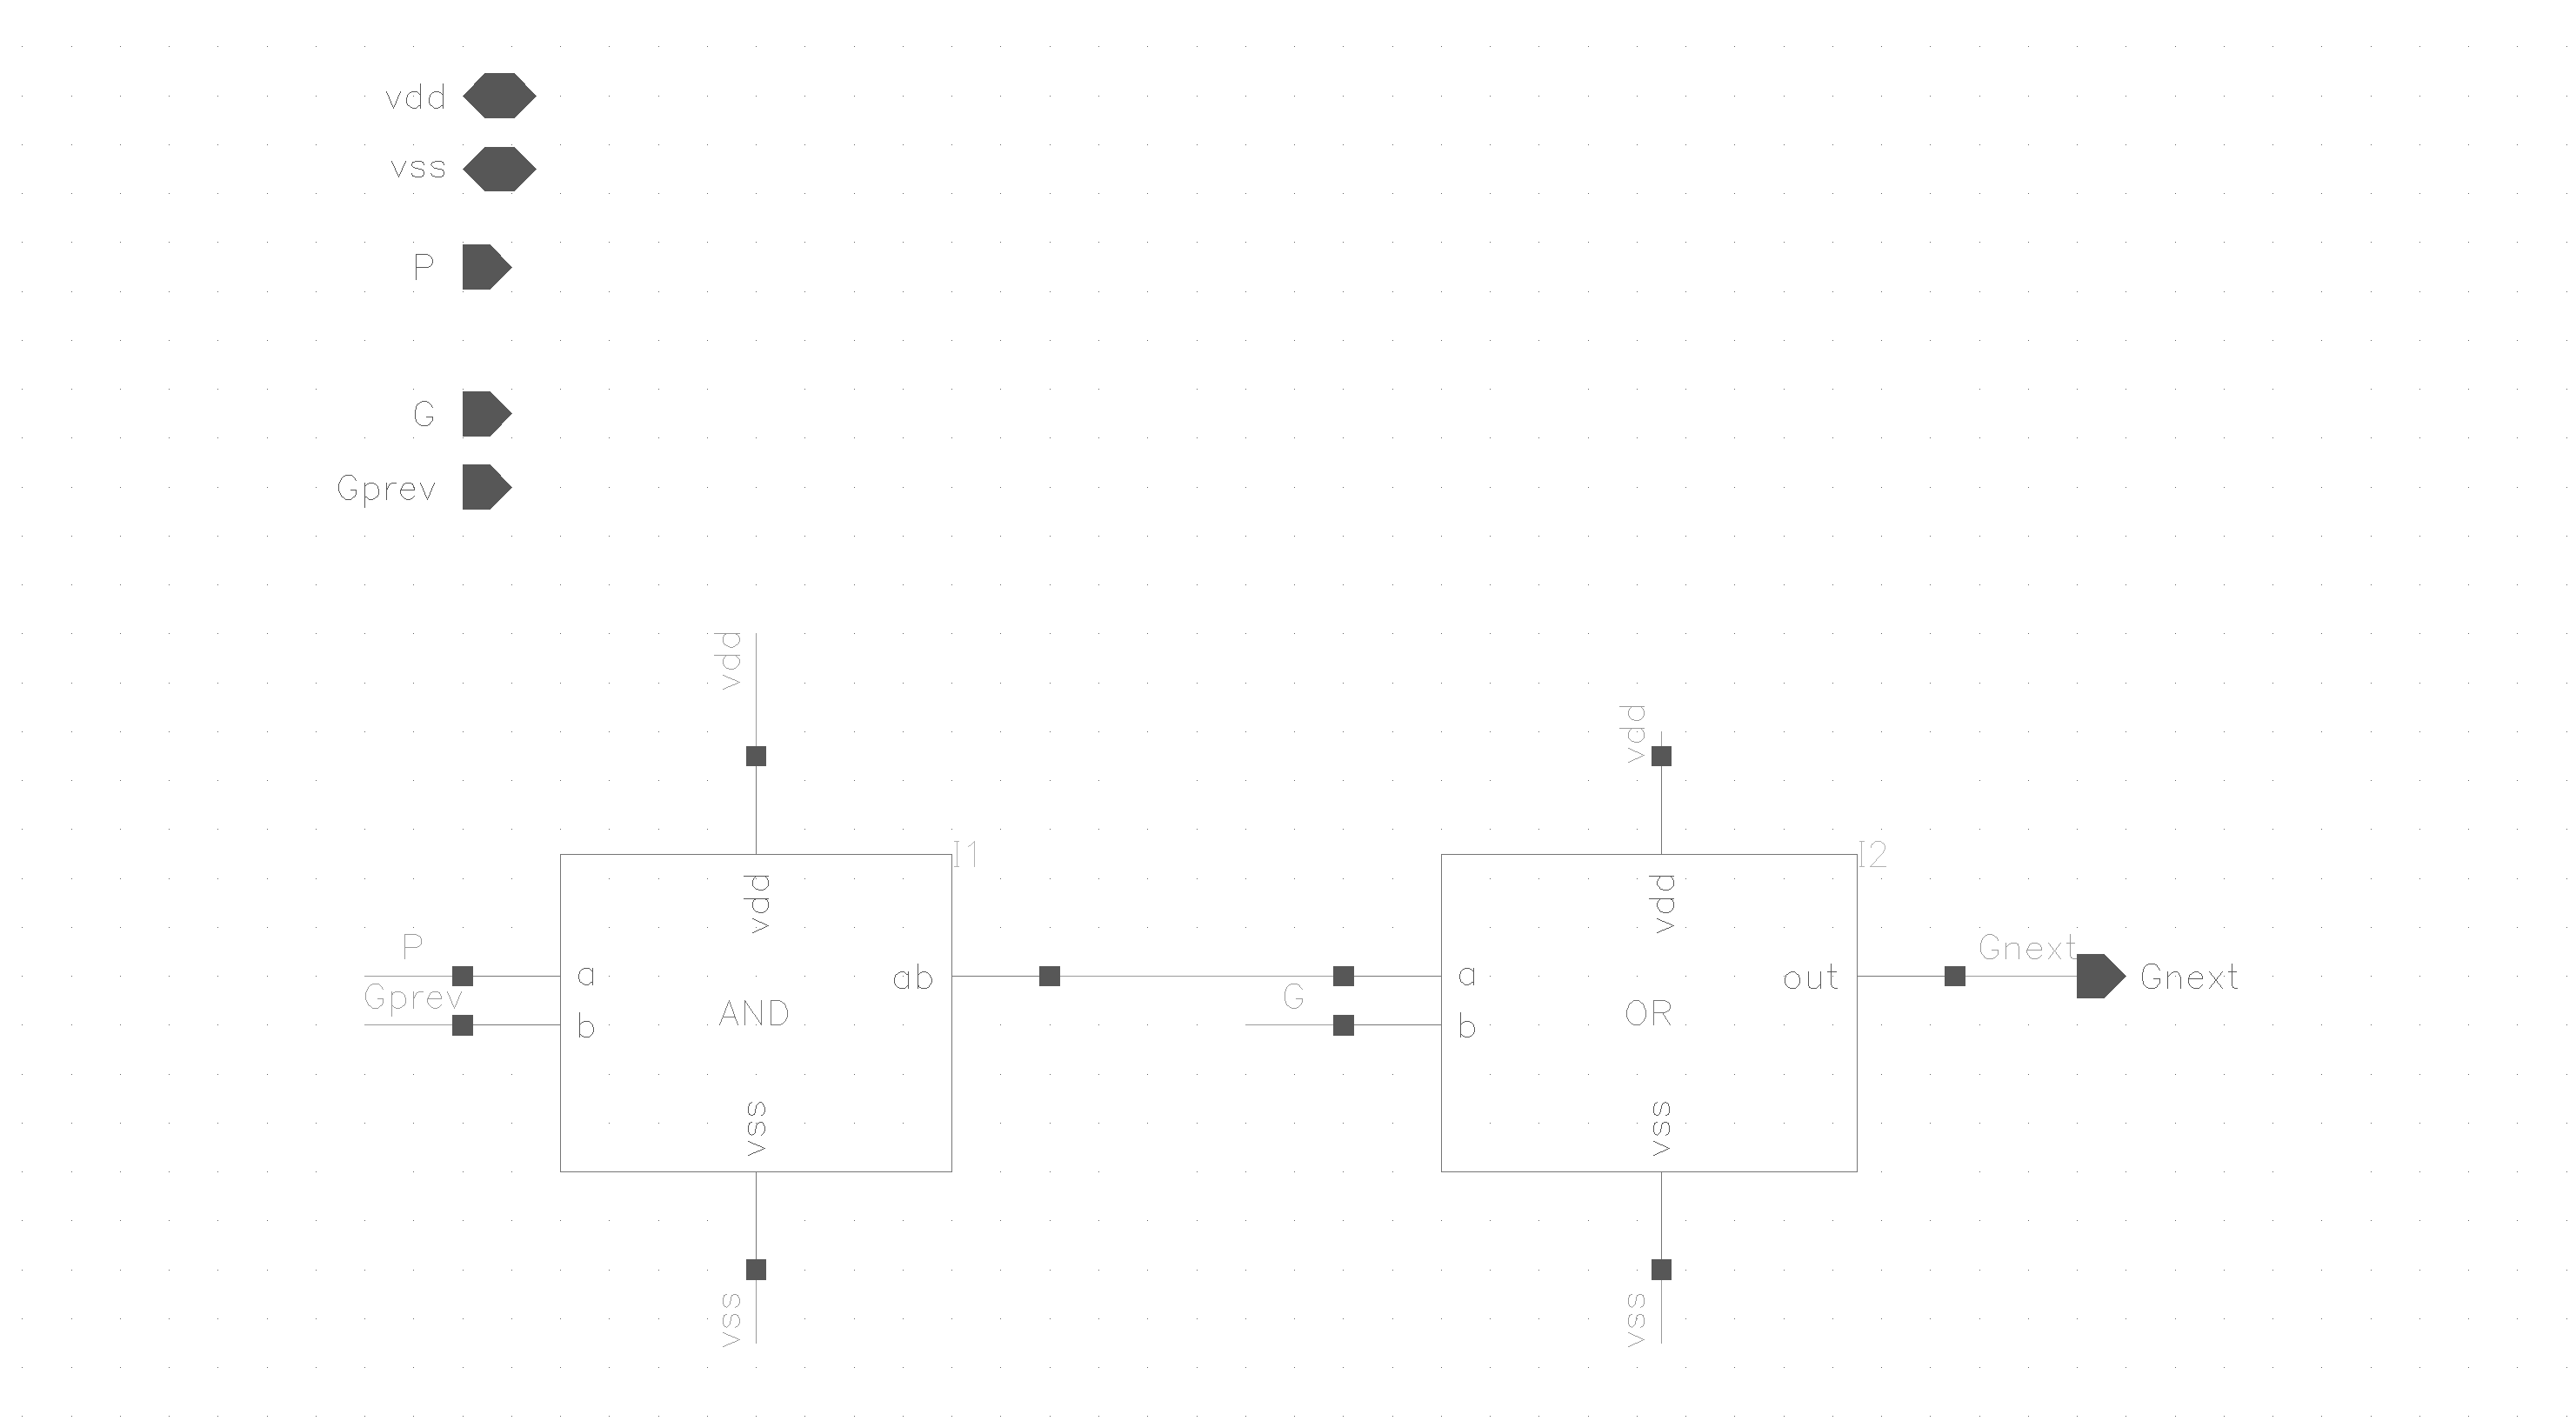
\includegraphics[width=1.2\textwidth]{../figures/yellow_carry}}
  \caption{Schematic view of the yellow carry block.} \label{fig:yellow_c}
\end{figure}

\begin{figure}[H]
  \centering
  \captionsetup{justification=centering}
  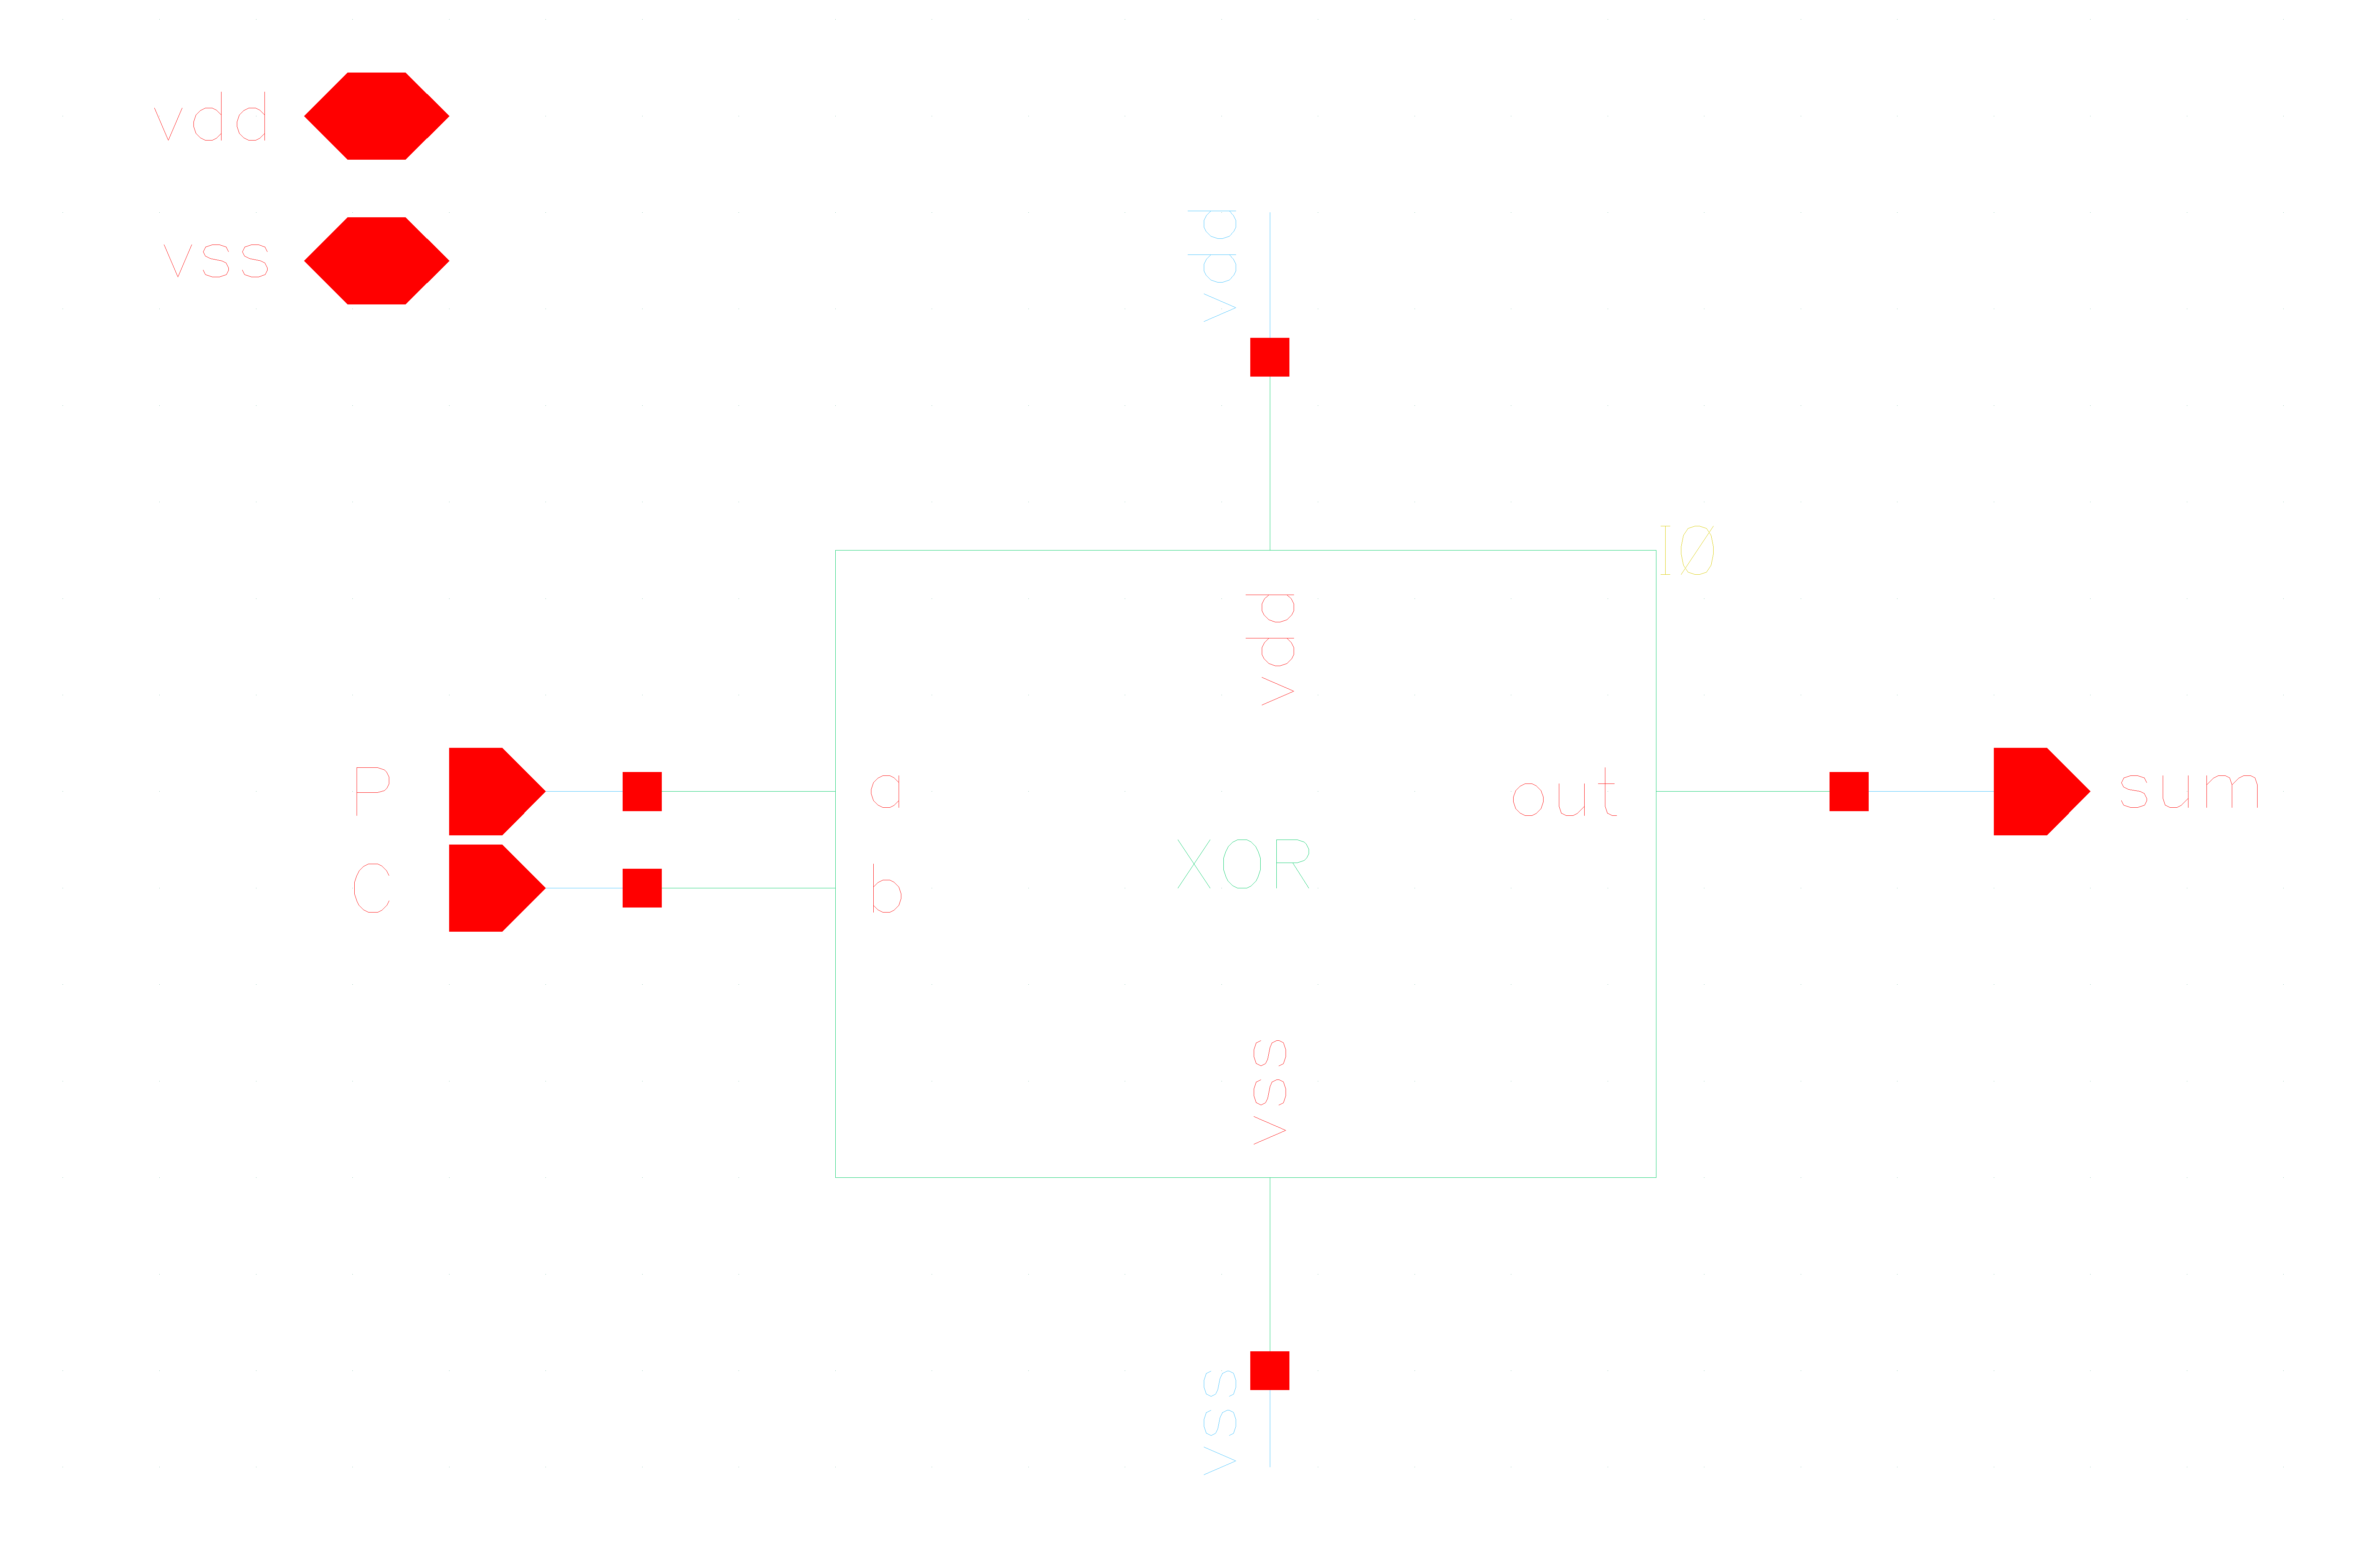
\includegraphics[clip,width=1.0\textwidth]{../figures/sum}
  \caption{Schematic view of the sum block.} \label{fig:sum}
\end{figure}

\subsection{Comparator}
The comparator consists of 17 2-input XNOR gates where one bit of each number is fed into each gate. The output from the XNOR gates are fed into a couple of AND gates which generates the final output. The comparator is 17 bits wide since it compares two 16 bit numbers plus their carry bits. The logic table of the XNOR gates is shown in table \ref{tab:xnor}.

\begin{table}[H]
  \caption{Logic table of XNOR block.}
  \centering
  \begin{tabular}{cc|c}
    \toprule
    $A_i$ & $B_i$ & $Y = \overline{(A_i \oplus B_i)}$ \\
    \midrule
    0 & 0 & 1 \\
    0 & 1 & 0 \\
    1 & 0 & 0 \\
    1 & 1 & 1 \\
    \bottomrule
    \label{tab:xnor}
  \end{tabular}
\end{table}
